\begin{figure*}[t]
\centering
\begin{subfigure}{0.48\textwidth}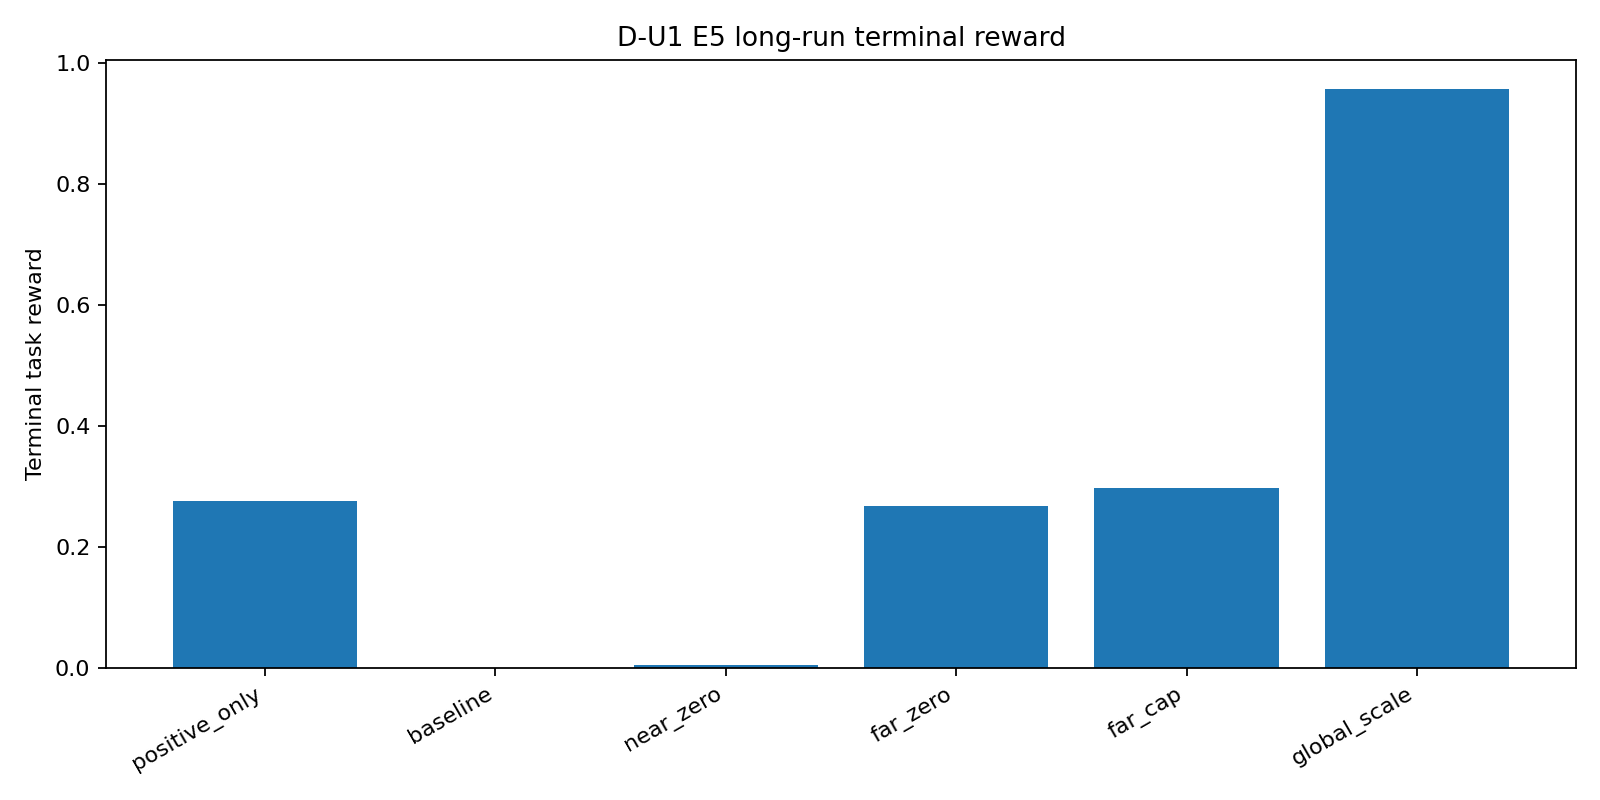
\includegraphics[width=\linewidth]{figures/generated/causal_terminal_reward.png}\caption{Terminal reward.}\end{subfigure}\hfill
\begin{subfigure}{0.48\textwidth}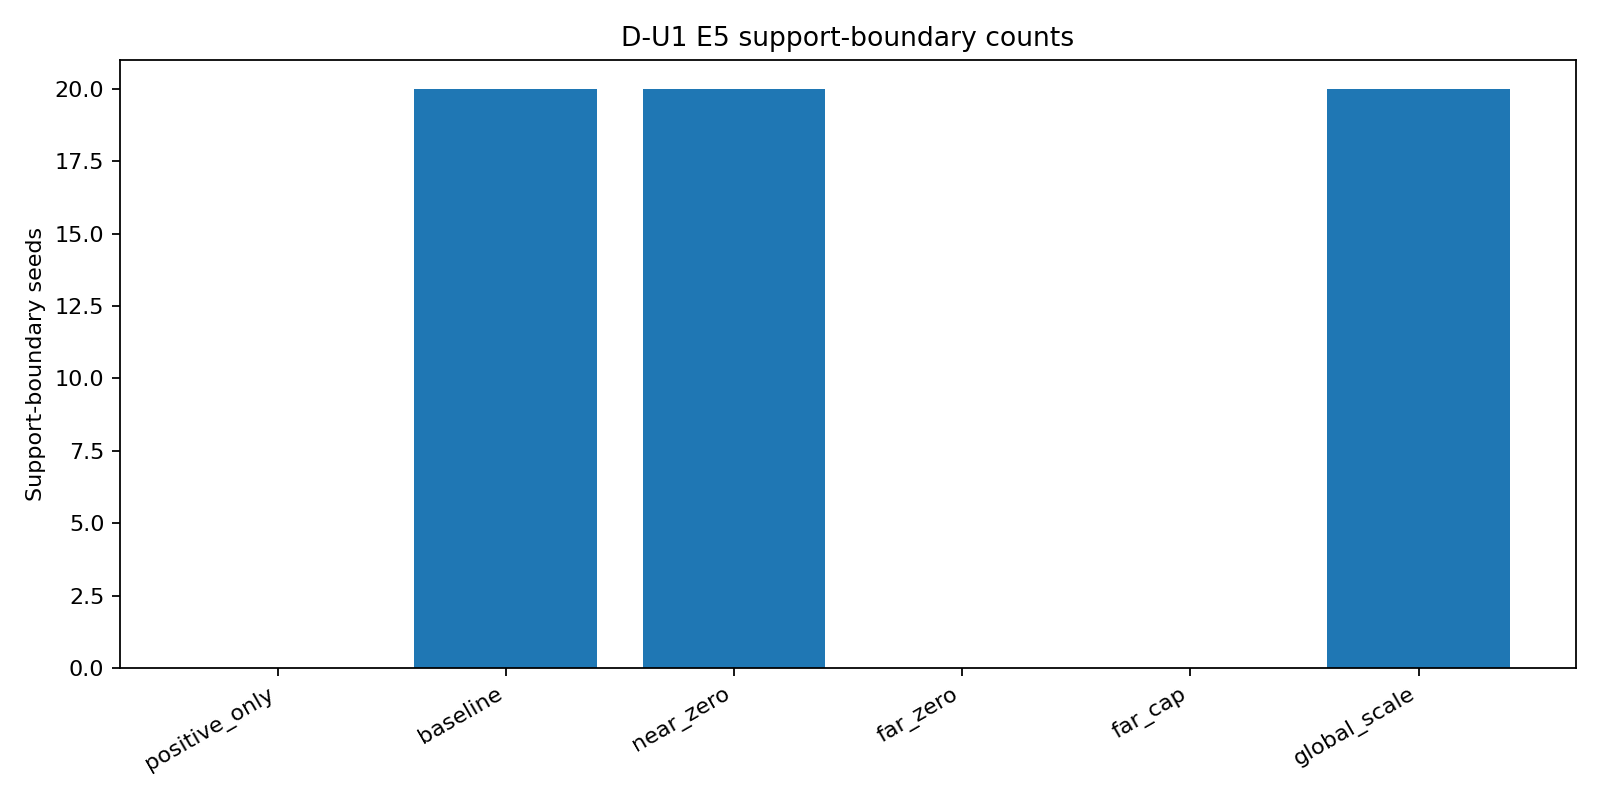
\includegraphics[width=\linewidth]{figures/generated/causal_support_boundary.png}\caption{Support-boundary events.}\end{subfigure}
\caption{D-U1 long-run causal results. Baseline and Near-zero preserve the rare/far negative pathway and reach the support boundary in 20/20 seeds; Far-zero and Far-cap remain bounded in 20/20 seeds. Global scaling can preserve task reward while still reaching the support boundary, illustrating why task, boundary, and numerical events must be reported separately.}
\label{fig:du1-causal}
\end{figure*}
\begin{table}[t]
\centering\small
\caption{D-U1 E5 long-run summary.}
\label{tab:du1-e5}
\begin{tabular}{lccc}
\toprule Method & Reward & Task collapse & Boundary \\
\midrule
baseline & 0.001 & 20/20 & 20/20 \\
near-zero & 0.006 & 20/20 & 20/20 \\
far-zero & 0.267 & 0/20 & 0/20 \\
far-cap & 0.297 & 0/20 & 0/20 \\
global-scale & 0.957 & 0/20 & 20/20 \\
positive-only & 0.275 & 0/20 & 0/20 \\
\bottomrule
\end{tabular}
\end{table}
